%! TEX program = pdflatex

\documentclass[oneside,solution]{karazin-complan-assign}

\usepackage[utf8]{inputenc}
\usepackage[english,ukrainian]{babel}

\usepackage{mathtools}

\let\Im\relax
\DeclareMathOperator{\Im}{Im}
\let\Re\relax
\DeclareMathOperator{\Re}{Re}

\usetikzlibrary{decorations.markings,positioning}

\providecommand{\poles}{
  \node (poles) at (2.5,1.5) {poles of $h(p_0)$};
  \draw[fill]
  (1.5,3) coordinate [circle,fill,inner sep=1pt,label=right:$p_1$] (p1)
  (2,-2) coordinate [circle,fill,inner sep=1pt,label=below:$p_2$] (p2)
  (-3,1) coordinate [circle,fill,inner sep=1pt,label=above:$p_3$] (p3)
  (-2,-1.5) coordinate [circle,fill,inner sep=1pt,label=above:$p_4$] (p4);
  \draw[ultra thin,gray] (poles) -- (p1) (poles) -- (p2) (poles.west) -- (p3) (poles) -- (p4);
}

\def\xr{3.5}
\def\yr{3}


\title{Домашня робота}
\author{Захаров Дмитро}
\studentID{МП-31}
\instructor{Гиря Н.П.}
\date{\today}
\duedate{23:59 7 квітня, 2024}
\assignno{2}
\semester{Весняний семестр 2024}
\mainproblem{Обчислення Інтегралів. Варіант 5}

\begin{document}

\maketitle

% \startsolution[print]

\problem{}

\textbf{Умова.} Обчислити інтеграл
\begin{equation*}
    \mathcal{I} = \int_{-\pi}^{+\pi} \frac{d\varphi}{3-2\sin\varphi}
\end{equation*}

\textbf{Розв'язання.} Зробимо заміну змінних $z=e^{i\varphi}$. Тоді, коли $\varphi$ пробігає від $-\pi$ до $+\pi$, то $z(\varphi)$ описує одиничне коло $\partial\mathcal{D}=\{z \in \mathbb{C}: |z| = 1\}$. Тому наша область інтегрування замінюється саме на одиничне коло. 

Тепер, виразимо $d\varphi$ та $\sin \varphi$ через $dz$ та $z$:
\begin{equation}
    z = e^{i\varphi} \implies dz = ie^{i\varphi}d\varphi \implies d\varphi = \frac{dz}{ie^{i\varphi}} = \frac{dz}{iz}
\end{equation}
\begin{equation}
    \sin \varphi = \frac{e^{i\varphi} - e^{-i\varphi}}{2i} = \frac{1}{2i}\left(z - \frac{1}{z}\right)
\end{equation}

Отже, маємо значення інтегралу
\begin{equation}
    \mathcal{I} = \oint_{|z|=1} \frac{dz}{iz\left(3 - 2 \cdot \frac{1}{2i}\left(z-\frac{1}{z}\right)\right)} = \oint_{|z|=1} \frac{dz}{-z^2 + 3iz + 1}
\end{equation}

Розглянемо підінтегральну функцію $f(z) = \frac{1}{-z^2+3iz + 1}$. За основною теоремою про лишки, цей інтеграл ми можемо знайти як $2\pi i \sum_k \text{Res}_{z=z_k}f(z)$, де сума береться по внутрішнім особливим точкам $z_k$. 

Отже, знаходимо лишки в особливих точках. Знайдемо нулі знаменника. Для цього треба знайти розв'язки  $-z^2+3iz+1 = 0$, звідки $z = \frac{-3i \pm \sqrt{-9+4}}{-2}$. Отже, маємо два полюси першого порядку: $z_1=\frac{(3-\sqrt{5})i}{2},z_2 = \frac{(3+\sqrt{5})i}{2}$. Помітимо, що оскільки $\frac{3+\sqrt{5}}{2} > 1$, то $z_2$ не належить одиничному кругу $\mathcal{D}$. В свою чергу, $z_1$ дійсно йому належить, оскільки:
\begin{equation}
    \underbrace{\frac{3-\sqrt{9}}{2}}_{=0} < \text{Im}(z_1) < \underbrace{\frac{3-\sqrt{4}}{2}}_{=\frac{1}{2}}, \; \text{Re}(z_1) = 0
\end{equation}

Отже, лишок можемо знайти як:
\begin{gather}
    \mathcal{I}=\oint_{|z|=1}f(z)dz = 2\pi i \cdot  \text{Res}_{z=z_1}f(z) = 2\pi i \cdot \frac{1}{(-z^2+3iz+1)'}\Big|_{z=z_1} \nonumber \\
    = 2\pi i \cdot \frac{1}{-2z_1+3i} = 2\pi i \cdot \frac{1}{\sqrt{5}i - 3i + 3i} = 2\pi i \cdot \frac{1}{\sqrt{5}i} = \frac{2\pi}{\sqrt{5}}
\end{gather}

Отже, остаточно $\boxed{\mathcal{I} = \frac{2\pi}{\sqrt{5}}}$.

\textbf{Відповідь.} $\frac{2\pi}{\sqrt{5}}$. 

\problem{}

\textbf{Умова.} Обчислити інтеграл
\begin{equation*}
    \mathcal{I} = \int_{-\infty}^{+\infty} \frac{dx}{x^2+2ix+2}
\end{equation*}

\textbf{Розв'язання.} Для обчислення цього інтегралу введемо допоміжний контур $\gamma$ наступним чином (він зображений на Рисунку \ref{fig:contour}):
\begin{gather}
    \gamma := I_R \cup \gamma_R, \\ I_R := [-R,R], \; \gamma_R := \{z \in \mathbb{C}: |z| = R \wedge \text{Im}(z) > 0\}
\end{gather}

Таким чином, розглядаємо допоміжний інтеграл
\begin{equation}
    \mathcal{I}_{\gamma} = \oint_{\gamma} f(z)dz, \; f(z) = \frac{dz}{z^2 + 2iz + 2}
\end{equation}

Розглянемо, чому він дійсно нам допоможе. Помітимо, шо оскільки $\gamma = I_R \cup \gamma_R$, то
\begin{equation}
    \mathcal{I}_{\gamma} = \int_{I_R} f(x)dx + \int_{\gamma_R} f(z)dz = \int_{-R}^{+R} f(x)dx + \int_{\gamma_R} f(z)dz
\end{equation}

\begin{figure}
    \centering
    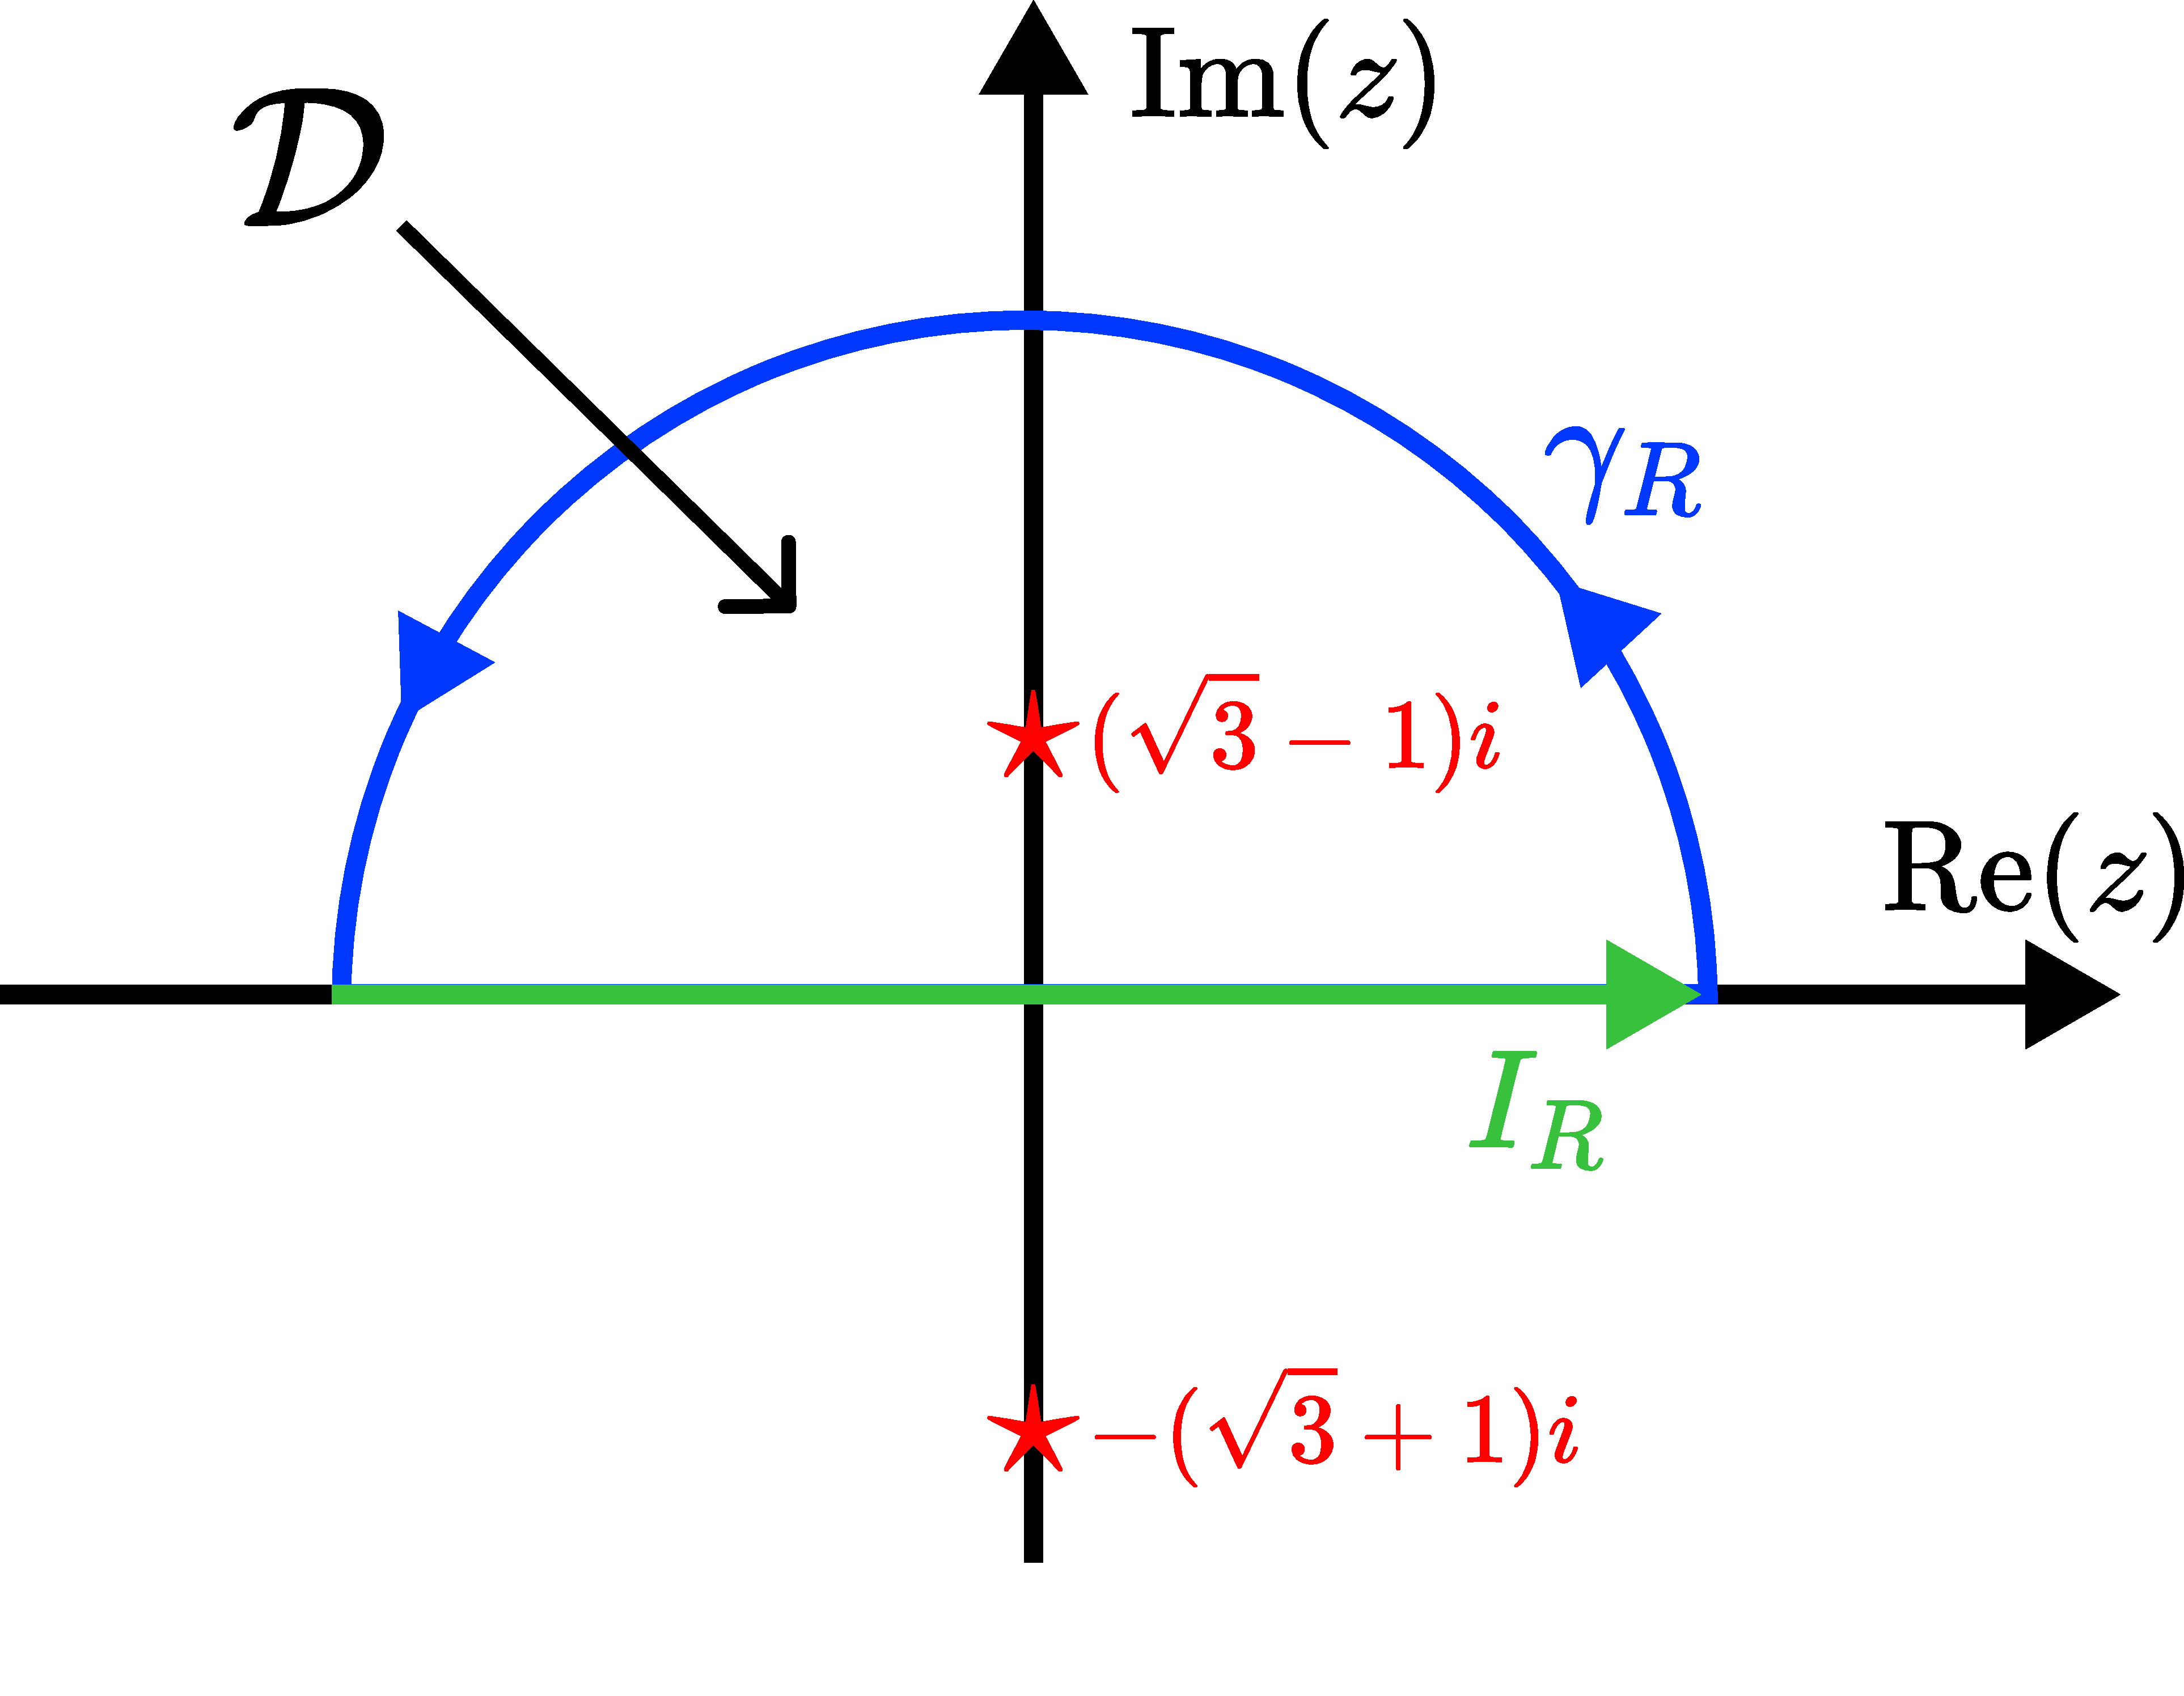
\includegraphics[width=0.6\textwidth]{images/hw_2/contour.pdf}
    \caption{Контур $\gamma$ в задачі 2 з особливими точками $f(z) = \frac{1}{z^2+2iz+2}$.}
    \label{fig:contour}
\end{figure}

Далі, якщо перейдемо до границі $R \to +\infty$:
\begin{equation}
    \mathcal{I}_{\gamma} = \int_{-\infty}^{+\infty} f(x)dx + \lim_{R \to \infty}\int_{\gamma_R} f(z)dz = \mathcal{I} + \lim_{R \to \infty} \int_{\gamma_R} f(z)dz
\end{equation}

Отже, бачимо, що наш шуканий інтеграл $\mathcal{I} = \mathcal{I}_{\gamma} - \lim_{R \to \infty}\int_{\gamma_R}f(z)dz$. Головна ідея наступна -- ми покажемо, що $\lim_{R \to \infty}\int_{\gamma_R}f(z)dz=0$ і тому наш шуканий інтеграл $\mathcal{I}$ повністю збігається з допоміжним $\mathcal{I}_{\gamma}$. Отже, наш розв'язок складається з двох частин: по-перше, знаходження інтегралу $\mathcal{I}_{\gamma}$, а по-друге доведення, що $\lim_{R \to \infty}\int_{\gamma_R}f(z)dz=0$. 

\textbf{Крок 1. Знаходження $\mathcal{I}_{\gamma}$.} Знайдемо особливі точки $f(z)$. Для цього помітимо, що нулі знаменника $z=(-1 \pm \sqrt{3})i$ -- два полюси першого порядку. Помітимо, що з цих двох нулей лише $z=(\sqrt{3}-1)i$ належить нашому півколу (вважаємо $R$ достатньо великим). Отже, маємо
\begin{gather}
    \int_{\gamma} f(z)dz = 2\pi i \cdot \text{Res}_{z=(\sqrt{3}-1)i}f(z) = 2\pi i \cdot \frac{1}{(z^2+2iz+2)'}\Big|_{z=(\sqrt{3}-1)i} \nonumber \\
    = 2\pi i \cdot \frac{1}{2z + 2i}\Big|_{z=(\sqrt{3}-1)i} = \frac{\pi i}{\sqrt{3}i} = \frac{\pi}{\sqrt{3}}
\end{gather}

\textbf{Крок 2. Доведення $\lim_{R \to \infty}\int_{\gamma_R}f(z)dz=0$.} Оцінимо наш інтеграл:
\begin{equation}
    \left|\int_{\gamma_R} f(z)dz \right| \leq \pi R \sup_{z \in \gamma_R} |f(z)| = \pi R \cdot \sup_{z \in \gamma_R}\frac{1}{|z^2+2iz + 2|}
\end{equation}

Далі потрібно оцінити значення у знаменнику. Скористаємося тим фактом, що $\forall z, w \in \mathbb{C}: |z + w| \geq ||z|-|w||$. Отже,
\begin{equation}
    |(z^2+2)+2iz| \geq ||z^2+2| - |2iz|| \geq ||z|^2 - |2| - |2iz||
\end{equation}

Далі, оскільки $z \in \gamma_R$, то $|z| = R$, тому:
\begin{equation}
    \left|\int_{\gamma_R} f(z)dz \right| \leq \frac{\pi R }{|R^2 - 2R - 2|} \sim \frac{\pi}{R} \xrightarrow[R \to \infty]{} 0
\end{equation}

Отже, дійсно $\lim_{R \to \infty}\int_{\gamma_R}f(z)dz=0$. Тому, $\boxed{\mathcal{I} = \frac{\pi}{\sqrt{3}}}$.

\textbf{Відповідь.} $\mathcal{I} = \frac{\pi}{\sqrt{3}}$.
    
\end{document}
